
\subsubsection{\stid{2.08} HPCToolkit} 
\paragraph{Overview} 

The HPCToolkit project is working to develop performance measurement
and analysis tools to help ECP application, library, runtime, and tool
developers understand where and why their software does not fully
exploit hardware resources within and across nodes of extreme-scale
parallel systems. Key deliverables of the project are a suite of
software tools that developers need to measure and analyze the
performance of parallel software as it executes on existing ECP
testbeds and new technologies needed to measure and analyze
performance on forthcoming GPU-accelerated exascale systems.

To provide a foundation for performance measurement and analysis, the
project team is working with community stakeholders, including
standards committees, vendors, and open source developers to improve
hardware and software support for measurement and attribution of
application performance on extreme-scale parallel systems. The
project team has been engaging vendors to improve hardware support
for performance measurement in next-generation GPUs and working
with other software teams to design and integrate new capabilities
into operating systems, runtime systems, communication libraries, and
application frameworks that will enhance the ability of software
tools to accurately measure and attribute code performance on
extreme-scale parallel systems.  Using emerging hardware and software
interfaces for monitoring code performance on both CPUs and GPUs, the project team is
working to extend capabilities to measure and analyze computation, data movement,
communication, and I/O as a program executes to pinpoint scalability
bottlenecks, quantify resource consumption, and assess
inefficiencies.

\paragraph{Key  Challenges}

Today's fastest supercomputers and forthcoming exascale systems all
employ GPU-accelerated compute nodes. Almost all of the 
computational power of GPU-accelerated compute nodes comes from GPUs rather than CPUs.
GPU-accelerated compute nodes have complex memory hierarchies that include 
multiple memory technologies with different bandwidth and latency characteristics. In addition, 
GPU-accelerated compute nodes have non-uniform connections between memories and computational elements (CPUs and GPUs). 
Furthermore, the next three DOE supercomputers (Perlmutter, Aurora, and Frontier) will feature GPUs from different vendors (NVIDIA, Intel, and AMD). 
There are significant differences in the underlying organization of these GPUs as well as their hardware and software support for performance measurement. For
performance tools, the need to support multiple CPU and GPU architectures significantly increases tool complexity.  At the same time, the
complexity of applications is increasing dramatically as developers
struggle to expose billion-way parallelism, map computation onto
heterogeneous computing elements, and cope with the growing complexity
of memory hierarchies. While application developers can employ
abstractions to hide some of the complexity of emerging parallel
systems, performance tools must be intimately familiar with each of
the features added to these systems to improve performance or
efficiency, develop measurement and analysis techniques that assess
how well these features are being exploited, and then relate these
measurements back to software to create actionable feedback that will
guide developers to improve the performance, efficiency, and
scalability of their applications.

\paragraph{Solution Strategy}

Development of HPCToolkit as part of ECP is focused on preparing it
for production use at exascale by enhancing it in several ways. First,
the team is adding new capabilities to measure and analyze
interactions between software and key hardware subsystems in
extreme-scale platforms, including GPUs and the complex memory hierarchies on GPU-accelerated compute nodes. A major focus of this effort is developing new capabilities for 
measurement and analysis of performance on GPUs.
Second, the team is working to improve performance
attribution given optimized code for a large collection of complex node-level programming
models used by ECP developers, including 
vendor specific programming models such as CUDA, HIP, and Data Parallel C++,
open source community programming models such as OpenMP,
and template-based programming models developed at national laboratories such as LLNL's RAJA and Sandia's KOKKOS. To support
this effort, the project team is enhancing the Dyninst binary analysis
toolkit, which is also used by other ECP tools. A major focus of this effort 
is to support analysis of GPU binaries. Third, the team is
improving the scalability of HPCToolkit so that it can be used to
measure and analyze extreme-scale executions. Fourth, the project team
is working to improve the robustness of the tools across the range of
architectures used as ECP platforms. Finally, the project team will
work other ECP teams to ensure that they benefit from HPCToolkit's
capabilities to measure, analyze, attribute, and diagnose performance
issues on ECP testbeds and forthcoming exascale systems.

\newpage
\paragraph{Recent Progress}

\begin{itemize}

\item
The project team developed a unified GPU monitoring substrate that supports GPUs from different vendors.
Based on the GPU-independent substrate, the project team developed kernel level measurement, 
which refers to the capability of collecting summary metrics for kernel launches, memory copies, and synchronizations,
for NVIDIA, Intel and AMD GPUs.

\item
The project team refined fine-grained measurement, which refers to the capability of collecting metrics inside a kernel, such as metrics for a device function, a basic block, a source line, or even a machine instruction, Nvidia GPUs.
Figure~\ref{fig:hpctoolkit}(a) shows a calling context that spans both CPU and GPU for a benchmark code implemented using LLNL's RAJA template-based programming model.
The team is also investigating fine-grained measurement for Intel GPUs and discussing fine-grained measurement support for AMD GPUs with AMD.

\item
The project team enhanced HPCToolkit for collecting and visualizing traces of both CPU and GPU activity.
Figure~\ref{fig:hpctoolkit}(b) shows a trace of a 6-process GPU-accelerated execution of a recent snapshot of Nyx---an adaptive mesh, compressible cosmological hydrodynamics simulation code being developed as part of the DOE ECP ExaSky project. In the figure, CPU trace lines appear as continuous multi-colored bands running the  trace lines the width of the figure. GPU trace lines show large intervals of white, indicating idleness, or red, indicating costly, excess synchronization present in the prototype code measured.

\item
The project team developed a novel approach that utilizes both shared and distributed memory parallelism to analyze and aggregate sparse data representations of performance measurements from every rank, thread and GPU stream in a program execution. 

\item 
The project team improved the reliability of HPCToolkit's hpcrun for monitoring complex dynamic library loading and unloading and interacting with the application when other software tools are present.

\end{itemize}

\begin{figure}[t]
\captionsetup{width=.96\textwidth}
\begin{minipage}[t]{.48\textwidth}
\centering
\includegraphics[width=\textwidth]{projects/2.3.2-Tools/2.3.2.08-HPCToolkit/hpctoolkit-raja-perf}
\\(a)
\end{minipage}
\hfill
\begin{minipage}[t]{.48\textwidth}
\centering
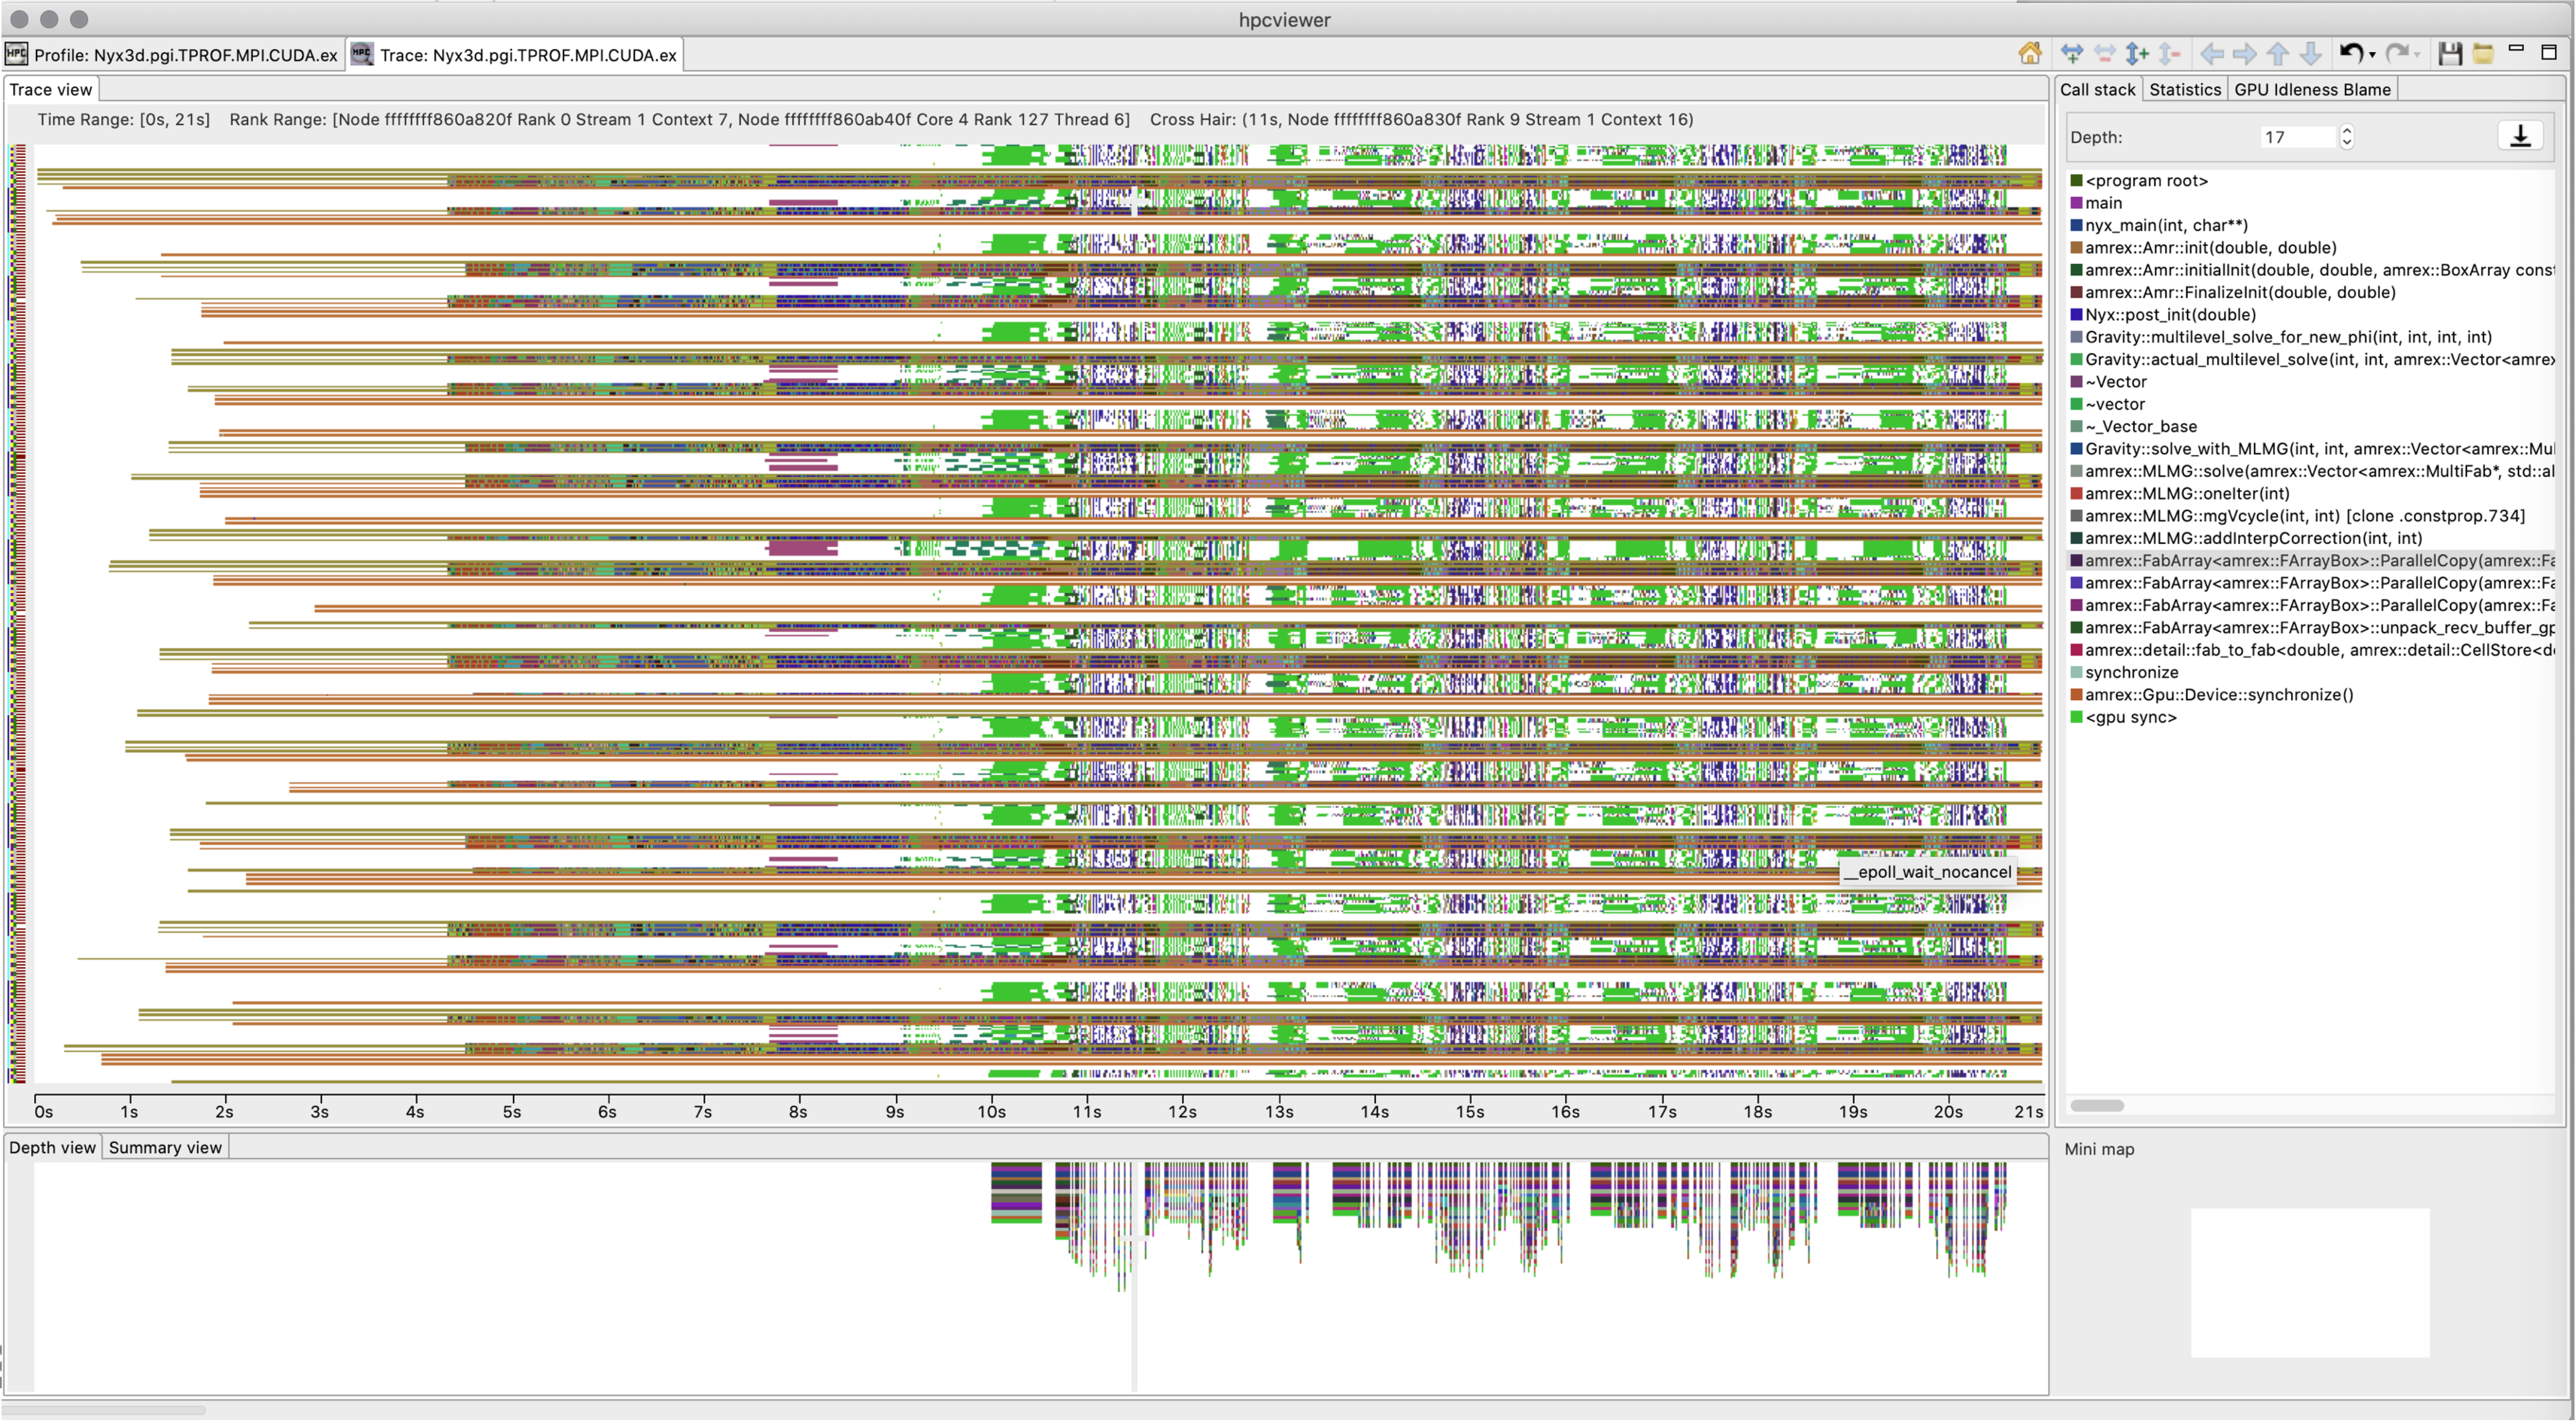
\includegraphics[width=\textwidth]{projects/2.3.2-Tools/2.3.2.08-HPCToolkit/hpctoolkit-nyx-trace}
\\(b)
\end{minipage}
\caption{(a) 
HPCToolkit's {\tt hpcviewer} showing a detailed attribution of GPU performance metrics in a 
profile of an optimized, GPU-accelerated benchmark written using LLNL's RAJA template-based programming model.
(b) HPCToolkit's {\tt hpctraceviewer} showing a 6-process GPU-accelerated execution trace of Nyx---an adaptive mesh, compressible cosmological hydrodynamics simulation code.}
\label{fig:hpctoolkit}
\end{figure}

\paragraph{Next Steps}
\begin{itemize}

\item 
Integrate GPU measurement and analysis capabilities into HPCToolkit's trunk for
release.

\item 
Continue to investigate solutions for fine-grained GPU performance measurement for Intel and AMD GPUs.

\item 
Continue to improve reliability of hpcrun for monitoring dynamic library loading and unloading

\item 
Work with the open source community to upstream GPU measurement support
developed by the project team into the community version of the {\tt
libomptarget} offloading library.

\item 
Work with DOE and platform vendors to evaluate and refine software interfaces for measuring GPU performance.

\end{itemize}
